%===========================
% Chapitre 2 : Données et Marchés de Crédit
%===========================
\chapter{Données en Finance de Crédit et Marchés de Prêts}
\label{chap:donnees_credit}
\textit{Enseigné par Julien Turc}

\section{Données et Fondamentaux du Crédit}

\subsection{Le défi de la basse fréquence et l'IA}
La stratégie quantitative appliquée au crédit se heurte à la rareté des données. Contrairement aux actions, les instruments de crédit (obligations, CDS, prêts) relèvent de la \textbf{basse fréquence} (\textit{low frequency}). Les séries temporelles sont courtes, souvent discontinues et limitent drastiquement l'application des méthodes d'intelligence artificielle classique. 

\begin{remarque}
Un \textit{dataset} multi-actifs robuste ne commence véritablement qu'entre \textbf{1990 et 1994}. Avec une trentaine d'années d'historique, le marché du crédit est très éloigné du paradigme \textit{big data}.
\end{remarque}

La disponibilité varie fortement selon les actifs et la géographie :
\begin{itemize}
    \item \textbf{Actions et obligations américaines} : Séries reconstruites jusqu'au début du XIX\textsuperscript{e} siècle (travaux de G. Baltussen). 
    \item \textbf{Ratings et défauts} : Les agences (Moody's, S\&P) fournissent des historiques précieux depuis le XIX\textsuperscript{e} siècle.
    \item \textbf{Dérivés et volatilité} : Les \textit{futures} naissent dans les années 1970. Le VIX (lancé en 1993) a pu être reconstruit jusqu'au krach de 1987.
    \item \textbf{Biais pré-2008} : Avant la standardisation réglementaire post-2008 (EMIR, MiFID II), les données souffrent d'une qualité inégale.
\end{itemize}

\begin{center}
\renewcommand{\arraystretch}{1.3}
\begin{tabular}{|l|c|p{5cm}|}
\hline
\textbf{Horizon / Segment} & \textbf{Fréquence des données} & \textbf{Applicabilité de l'IA} \\
\hline
Trading électronique (HFT) & Haute (ticks) & Maximale (Deep learning) \\
\hline
Crédit IG / High Yield & Basse (jours) & Limitée (risque de surapprentissage) \\
\hline
Investissement long terme & Jours/Mois & Faible (séries trop courtes) \\
\hline
\end{tabular}
\end{center}

\begin{remarque}
L'absence de \textit{big data} impose en crédit le recours à des approches économes en données : \textbf{modèles structurels} (Merton), modèles à \textbf{intensité de défaut} (formes réduites), modèles factoriels et cadres bayésiens incluant l'expertise humaine.
\end{remarque}

\subsection{Mécanismes de transfert de crédit}
Le marché du crédit englobe également les prêts bancaires (\textit{loans}). Leur propriété peut être transférée via trois mécanismes juridiques :

\begin{description}
    \item[La Novation :] L'ancien contrat est annulé et remplacé par un nouveau. Le repreneur assume les droits économiques et les obligations contractuelles. Le \textbf{consentement explicite de l'emprunteur} est obligatoire.
    \item[La Cession (\textit{Assignment}) :] Le prêteur transfère uniquement ses droits économiques (intérêts, principal) à un tiers et sort du contrat. L'emprunteur est notifié, mais son \textbf{consentement n'est généralement pas requis}.
    \item[La Sous-participation :] Accord bilatéral en coulisses. Le prêteur initial reste la seule contrepartie officielle de l'emprunteur. Le sous-participant finance le prêt et en touche les flux, assumant le risque de défaut à hauteur de son apport. L'emprunteur n'est \textbf{ni informé, ni impliqué}.
\end{description}

\begin{center}
\renewcommand{\arraystretch}{1.2}
\begin{tabular}{|l|c|c|c|}
\hline
\textbf{Critère} & \textbf{Novation} & \textbf{Cession} & \textbf{Sous-participation} \\
\hline
Accord de l'emprunteur & Obligatoire & Souvent non requis & Non requis \\
\hline
Transfert des droits & Oui & Oui & Partiel (économique) \\
\hline
Transfert des obligations & Oui & Non & Non \\
\hline
L'emprunteur est informé & Oui & Oui (notification) & Non \\
\hline
Nouveau contrat créé & Oui & Non (avenant) & Non (accord bilatéral) \\
\hline
\end{tabular}
\end{center}

\subsection{Cadre Juridique et Faillites : États-Unis vs Europe}
L'impact et la gestion d'un défaut varient drastiquement selon la culture juridique.

\begin{itemize}
    \item \textbf{Le Chapter 11 américain} : Historiquement très favorable à l'entreprise (\textit{debtor-friendly}). Il permet à une société de se déclarer en faillite de manière stratégique pour geler ses dettes, restructurer ses obligations sociales (retraites, licenciements) et repartir sur des bases saines (ex: compagnies aériennes). Bien que l'événement de crédit soit déclenché (déclenchement des CDS), l'entreprise survit souvent.
    \item \textbf{Le Modèle Européen} : La priorité est souvent la préservation de l'emploi et de l'activité, mais via des procédures judiciaires lourdes et longues (10 à 20 ans). 
    \begin{itemize}
        \item Inconvénient : Les capitaux sont bloqués longtemps.
        \item Avantage : Les taux de recouvrement (\textit{Recovery Rates}) finaux ont tendance à être plus élevés qu'aux US, et les taux de défaut bruts historiquement plus faibles.
    \end{itemize}
\end{itemize}

\section{Modélisation Quantitative du Risque de Crédit}

La modélisation du risque de crédit se heurte à une difficulté fondamentale : la présence de deux variables sous-jacentes distinctes, à savoir le spread de crédit (variable de marché continue) et le risque de défaut (événement discret).

\subsection{Approche Structurelle : Le Modèle de Merton (1973)}
\label{sec:merton}

Le modèle de Black-Scholes-Merton révolutionne l'analyse en concevant les obligations comme des \textbf{produits dérivés sur la valeur des actifs de l'entreprise ($V_t$)}. 

Pour une dette de nominal $K$ à maturité $T$, le créancier possède l'équivalent d'un \textbf{zéro-coupon sans risque minoré d'un Put vendu} sur l'entreprise :
\begin{itemize}
    \item \textbf{Solvabilité} ($V_T \geq K$) : La dette est remboursée. Le créancier touche $K$ (pas d'\textit{upside}).
    \item \textbf{Défaut} ($V_T < K$) : Le créancier récupère les actifs $V_T$. Il subit une perte équivalente au paiement d'un Put exercé contre lui.
\end{itemize}

Le flux de remboursement s'écrit formellement :
\begin{equation}
    \min(V_T, K) = K - \max(K - V_T, 0)
\end{equation}

\begin{definition}[Cadre mathématique de Merton]
Dynamique des actifs (Mouvement Brownien Géométrique) : 
\[ dV_t = \mu V_t \, dt + \sigma V_t \, dW_t \]
L'action (\textit{equity}) est modélisée comme un \textbf{Call} de strike $K$ sur $V_T$ : 
\[ E_t = \mathbb{E}^{\mathbb{Q}}\!\left[e^{-r(T-t)} \max(V_T - K, 0)\right] \]
Par parité Call-Put, la dette risquée vaut : 
\[ D_t = V_t - E_t \]
\end{definition}

\textbf{Lien avec la physique} : Ce modèle repose sur un \textbf{portefeuille d'autofinancement} (couverture en delta) sans opportunité d'arbitrage. L'équation aux dérivées partielles (EDP) qui en résulte peut se ramener, par changement de variables, à \textbf{l'équation de la chaleur} de Fourier, ce qui permet d'obtenir une formule fermée explicite.

\subsection{Approches à Intensité : Processus de Défaut}

Contrairement aux variations continues des prix d'actifs (mouvement brownien), le défaut s'apparente à un processus de sauts (\textit{jump process}), comparable à une météorite tombant de manière soudaine et imprévisible.

\begin{itemize}
    \item \textbf{Cadre de Monique Jeanblanc} : Pour pallier la rigidité des modèles structurels (Type Merton), la chercheuse Monique Jeanblanc a formalisé un cadre mathématique plus flexible. Ce modèle sépare la filtration globale (information de marché) de la filtration du défaut (information abrupte de l'événement), permettant de traiter le défaut comme un temps d'arrêt totalement inaccessible.
    \item \textbf{Processus de Cox} : En pratique, on utilise les processus de Cox (ou processus de Poisson doublement stochastiques). Le défaut est piloté par une \textbf{intensité stochastique} $\lambda_t$, représentant la probabilité instantanée de défaut conditionnelle à l'information disponible.
    \begin{remarque}
    Une anomalie mathématique de ce cadre est que l'intensité $\lambda_t$ peut continuer à se diffuser mathématiquement même après que l'entreprise a fait défaut, ce qui nécessite des ajustements dans la valorisation (arrêt du processus à $\tau$).
    \end{remarque}
\end{itemize}

\subsection{Philosophie de Valorisation et Incomplétude}
Contrairement aux marchés actions (modélisés par Black-Scholes), le marché du crédit est fondamentalement \textbf{incomplet}.

\begin{itemize}
    \item \textbf{Absence de couverture parfaite} : Dans le modèle de Black-Scholes, une option peut être répliquée parfaitement par une stratégie auto-finançante (delta-hedging). En crédit, cette réplication est impossible (illiquidité, sauts de défaut).
    \item \textbf{Probabilité Risque Neutre ($\mathbb{Q}$) vs Historique ($\mathbb{P}$)} : 
    \begin{itemize}
        \item Dans les modèles actions (ex: Dupire), on calibre les probabilités risque-neutre sur les prix des options liquides.
        \item En crédit, l'approche est souvent plus \textbf{actuarielle} (estimation des pertes attendues selon $\mathbb{P}$) faute de liquidité suffisante pour une calibration purement $\mathbb{Q}$.
    \end{itemize}
    \item \textbf{L'arbitrage fondamental} : Il existe un arbitrage structurel entre le spread des tranches de CDO et le spread moyen du collatéral. Le profit se concentre souvent sur la tranche \textbf{Mezzanine}, point de rencontre des investisseurs sophistiqués.
\end{itemize}

\subsection{La Copule Gaussienne et ses limites}
Pour valoriser (pricer) ces paniers de crédits corrélés, le marché a adopté le modèle de la \textbf{Copule Gaussienne} (David Li), qui agrège les probabilités marginales de défaut via une matrice de corrélation simple.

\begin{itemize}
    \item \textbf{La Faille} : C'est un modèle statique et purement probabiliste. Il donne un prix à un instant $t$, mais ne fournit pas de stratégie de couverture dynamique (\textit{greeks} instables).
    \item \textbf{Convexité négative des tranches Senior} : Les tranches \textit{Super Senior} sont \textit{short volatilité} et \textit{short corrélation}. Elles offrent un faible rendement mais portent un \textbf{risque de queue} (tail risk) catastrophique : si la corrélation des défauts bondit (crise systémique), ces tranches censées être sûres s'effondrent.
    \item \textbf{CDO-squared (CDO$^2$)} : Pour booster les rendements avant 2007, on a créé des "CDO de CDO" (re-titrisation de tranches Mezzanine). Cette structure a démultiplié l'exposition à la corrélation : lors du retournement du marché, l'effet de levier sur la corrélation a provoqué des défauts simultanés massifs.
\end{itemize}

\section{Titrisation, Produits Structurés et Alchimie Financière}

\subsection{Du Crédit Privé à la Titrisation}
Le marché du crédit s'est fortement orienté vers le domaine privé (Private Credit). Contrairement aux marchés publics, ces prêts manquent de liquidité. En 1989, le Comité de Bâle instaure des contraintes de capital pour les banques. Pour alléger leur bilan et libérer du capital réglementaire, les banques ont recours à la \textbf{titrisation} via des SPV (Special Purpose Vehicle).

\begin{figure}[htbp]
    \centering
    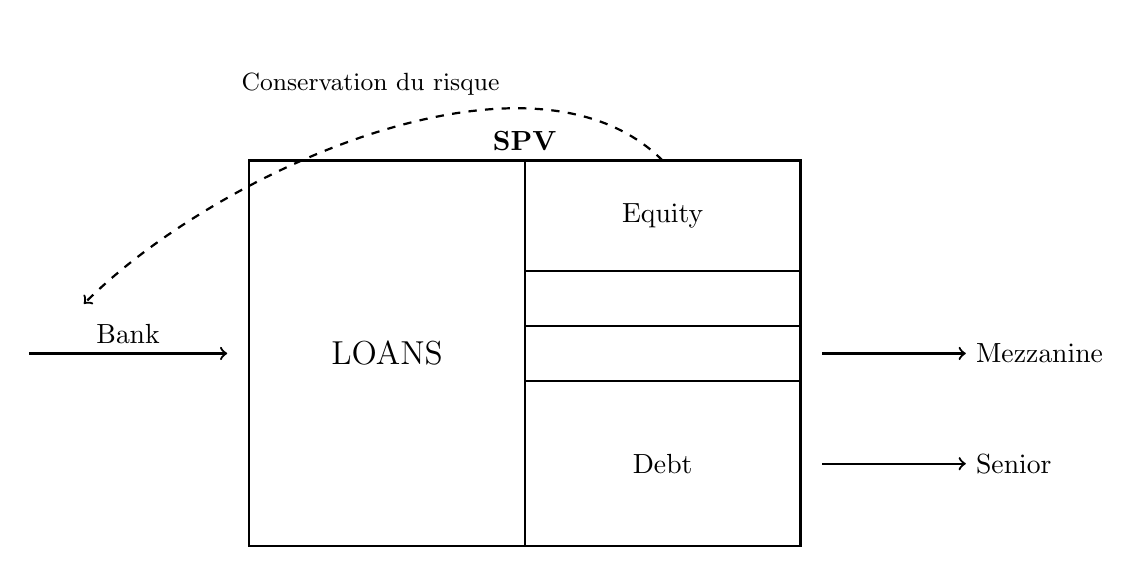
\begin{tikzpicture}[scale=1.4]
        % SPV Box (Wider and Taller)
        \draw[thick] (0,0) rectangle (5,3.5);
        \draw[thick] (2.5,0) -- (2.5,3.5);
        \node[above] at (2.5, 3.5) {\textbf{SPV}};
        
        % Left side (Assets)
        \node at (1.25, 1.75) {\large LOANS};
        \draw[->, thick] (-2, 1.75) -- (-0.2, 1.75) node[midway, above] {Bank};
        
        % Right side (Liabilities)
        \draw[thick] (2.5, 2.5) -- (5, 2.5);
        \node at (3.75, 3) {Equity};
        
        % Mezzanine tranches
        \draw[thick] (2.5, 2.0) -- (5, 2.0);
        \draw[thick] (2.5, 1.5) -- (5, 1.5);
        
        \node at (3.75, 0.75) {Debt};
        
        % Arrows for tranches (More spacing)
        \draw[->, thick] (5.2, 1.75) -- (6.5, 1.75) node[right] {Mezzanine};
        \draw[->, thick] (5.2, 0.75) -- (6.5, 0.75) node[right] {Senior};
        
        % Arrow back to bank (Bank retains equity) - flatter curve
        \draw[->, thick, dashed] (3.75, 3.5) to[out=135, in=45, looseness=0.8] (-1.5, 2.2);
        \node[above, font=\small] at (1.1, 4.0) {Conservation du risque};
    \end{tikzpicture}
    \caption{Structure de bilan d'un SPV de Titrisation}
    \label{fig:spv_structure}
\end{figure}

L'industrie financière a cherché à recycler des dettes risquées (CBO, CLO) pour créer des produits de haute qualité. L'objectif est de transformer des actifs de qualité médiocre (ex: \textit{Junk bonds}) en passifs notés \textit{Investment Grade} (voire AAA) grâce à la structuration. C'est une forme d'alchimie financière transformant le plomb (dettes risquées) en or (tranches Senior AAA).

\subsection{Structuration Avancée et Rôle des Agences}
Le rôle du structurateur est d'optimiser la découpe des tranches pour maximiser la valeur créée.
\begin{itemize}
    \item \textbf{Dimensionnement de l'Equity} : L'enjeu est de minimiser la taille de la tranche \textit{Equity} (la plus risquée et la plus coûteuse en capital) tout en assurant que les tranches \textit{Senior} obtiennent la notation cible (AAA ou AA).
    \item \textbf{Processus itératif} : Le structurateur ajuste les points d'attachement. Si la notation cible n'est pas atteinte par les agences, il doit "épaissir" la tranche inférieure (augmenter le rehaussement de crédit).
\end{itemize}

Les agences de notation modélisent la distribution des pertes du portefeuille $\mathbb{P}[\text{Loss} \ge x]$.

\begin{figure}[htbp]
    \centering
    \begin{tikzpicture}[scale=1.4]
        % Axes - extended x-axis for better label spacing
        \draw[->, thick] (0,0) -- (7,0) node[right] {$x$};
        \draw[->, thick] (0,0) -- (0,4) node[above] {$\mathbb{P}[\text{Loss} \ge x]$};
        
        % Labels
        \node[left] at (0,3.5) {$100\%$};
        \node[below] at (5.5,0) {$100$};
        \node[below left] at (0,0) {$0$};
        
        % Box limit
        \draw[gray, thin] (0,3.5) -- (5.5,3.5) -- (5.5,0);
        
        % Survival Curve
        \draw[thick] (0,3) .. controls (1.5,2.5) and (2,1) .. (4.5,0.1);
        
        % Tranching lines (Red as on chalkboard)
        \draw[dashed, red, thick] (1.5,0) -- (1.5,2);
        \draw[dashed, red, thick] (2.8,0) -- (2.8,1);
        
        % Arrows for attachment/detachment points - stagger labels vertically to avoid overlap
        
        % Equity
        \draw[<->, red, thick] (0,-0.3) -- (1.5,-0.3);
        \node[below, red, font=\small] at (0.75, -0.3) {Equity};
        
        % Mezzanine - shifted down slightly to not overlap if close
        \draw[<->, red, thick] (1.5,-0.3) -- (2.8,-0.3);
        \node[below, red, font=\small] at (2.15, -0.8) {Mezzanine};
        \draw[dotted, red] (2.15,-0.3) -- (2.15,-0.8); % guide line
        
        % Senior
        \draw[<->, red, thick] (2.8,-0.3) -- (5.5,-0.3);
        \node[below, red, font=\small] at (4.15, -0.3) {Senior};
    \end{tikzpicture}
    \caption{Distribution des pertes et points d'attachement des tranches}
    \label{fig:loss_distribution}
\end{figure}

Le graphique illustre comment le risque est découpé : la tranche \textit{Equity} encaisse les premières pertes. Les tranches \textit{Mezzanine} et \textit{Senior} ne sont touchées que si les pertes cumulées dépassent leurs seuils d'attachement respectifs.

\subsection{L'essor des CDO Synthétiques}
Face à la pénurie d'obligations physiques, le marché a muté vers les dérivés, créant les \textbf{CSO (Collateralized Synthetic Obligations)}.
\begin{itemize}
    \item \textbf{Transition vers le CDS} : Acheter/vendre l'obligation physique est coûteux. Le CDS permet de prendre une exposition synthétique efficace sans mobiliser la trésorerie nécessaire à l'achat du nominal.
    \item \textbf{Mécanisme} : Au lieu de détenir des obligations physiques, le SPV vend de la protection via des CDS à une banque. Les investisseurs touchent les primes des CDS. Cela a permis de créer de la dette "artificielle" à l'infini pour répondre à la demande mondiale de rendement.
\end{itemize}

\section{Perspective Historique et Enseignements des Crises}

\subsection{Les Premières Crises Souveraines et Bancaires}
\begin{itemize}
    \item \textbf{Crise polonaise (1980s)} : Emprunts en dollars et choc des taux de Volcker. Révélation du risque souverain en devises étrangères et de l'illiquidité.
    \item \textbf{Crise des Savings \& Loans (US, 1980s)} : Répression financière, prise de risque excessive dans l'immobilier/Junk bonds, et \textbf{risque de transformation} fatal (passifs courts vs actifs longs).
    \item \textbf{Plan Brady (1989)} : Création des \textit{Brady Bonds} (garantis par zéro-coupons US) pour purger les bilans bancaires, donnant naissance au marché secondaire liquide de la dette émergente.
\end{itemize}

\subsection{L'Éclatement de la Bulle Technologique et Fraudes}
Le début des années 2000 a mis en lumière les limites des notations de crédit.
\begin{itemize}
    \item \textbf{Crise des Télécoms (2001-2002)} : Endettement massif pour les licences 3G. La dégradation des ratings a créé des \textbf{Fallen Angels}, fermant brutalement l'accès au refinancement.
    \item \textbf{Faillites Idiosyncratiques et Fraudes} : Après la bulle internet, le marché a découvert le risque de \textbf{fraude massive} ("fraudes sèches") non corrélé à la macroéconomie.
    \begin{itemize}
        \item \textbf{Enron (2001)} : Pertes masquées via des SPV complexes.
        \item \textbf{Parmalat (2003)} : Trou de 14 milliards d'euros (faux comptes).
    \end{itemize}
\end{itemize}

\subsection{Leçons de la Gestion Moderne : LTCM et Crédit Privé}

L'effondrement du fonds \textit{Long Term Capital Management} (LTCM) en 1998 illustre les dangers de l'arbitrage à fort effet de levier (200:1). Malgré une "Dream Team" (Merton, Scholes), le fonds a implosé lors du défaut russe (Flight to Quality), prouvant que "le marché peut rester irrationnel plus longtemps que vous ne pouvez rester solvable".

\textbf{Le Crédit Privé Moderne} : Le passage de la gestion \textit{Buy-and-Hold} à la comptabilité \textit{Mark-to-Market} a introduit une volatilité artificielle. Aujourd'hui (2025-2026), le marché du \textit{Private Credit} présente, comme avant 2008, une opacité sur les risques réels et un danger majeur : le \textbf{Cliff Risk} ("risque de falaise"), où un produit structuré apparemment sûr perd toute sa valeur brutalement si la corrélation change.